% !TEX root = da.tex



\subsection{Landmarks for unsupervised domain adaptation}  \label{sLandmark}
One of the key challenges to unsupervised domain adaptation is that there is no labeled data in the target domain to train discriminative classifiers. We tackle this by the insight of landmarks --- some labeled instances in the source domain may be regarded as a subset drawn from the target. By automatically identifying those landmarks, we can thus approximate the discriminative loss of the target domain. 

As a motivating example for the landmarks, suppose the source domain contains furniture in a home environment  and the target domain consists of images of office-style furniture.  Conceivably, certain images from the source --- for instance those taken in home offices --- could also be regarded as samples from the target. Such images thus might have properties that are shared by both domains. These properties in turn can guide learning algorithms to search for invariant features or kernels.


%Our approach automatically identifies such images, which we call ``landmarks''.  We use them to bridge the source and target domains to generate multiple candidates of invariant feature spaces. Additionally, we exploit the {\em labels of the landmarks} to adapt the invariant features to be {\em discriminatively} optimal for the target domain, in contrast to GFK.  We also show that the landmark-based approach integrates well with GFK. In particular, our automatic landmark identification algorithm (section~\ref{sFindLandmark}) benefits significantly from using GFK as a similarity measure.

In the following, we give an overview of the landmark based approach, followed by details on how to identify landmarks. We then show how to exploit the landmarks for a series of GFKs and discriminative learning of kernels for the target domain.

\subsubsection{Overview of the landmark based approach to unsupervised adaptation}
As the first step, our landmark based approach plucks out and exploits the most desirable instances ---landmarks --- to facilitate adaptation. Identifying those instances requires comparing all possible subsets from the source domain to the target. We will show how this can be addressed with tractable optimization.

Leveraging the landmarks, we create a cohort of auxiliary tasks where landmarks explicitly bridge the source and target domains. Specifically, in those auxiliary tasks, the original target domain is augmented with landmarks, blurring the distinction across domains. Thus, those tasks are \emph{easier} to solve than the original domain adaptation problem. We show this is indeed true both theoretically and empirically. The auxiliary tasks offer multiple views of the original problem; they differ by how the landmarks are selected, which in turn are determined by the data pairwise similarities. In this work, we measure similarities at multiple scales (of distances). Thus, each task provides a different perspective to the adaptation problem, by being robust to idiosyncrasies in the domains at different granularities.


\begin{figure*}[t]
\centering
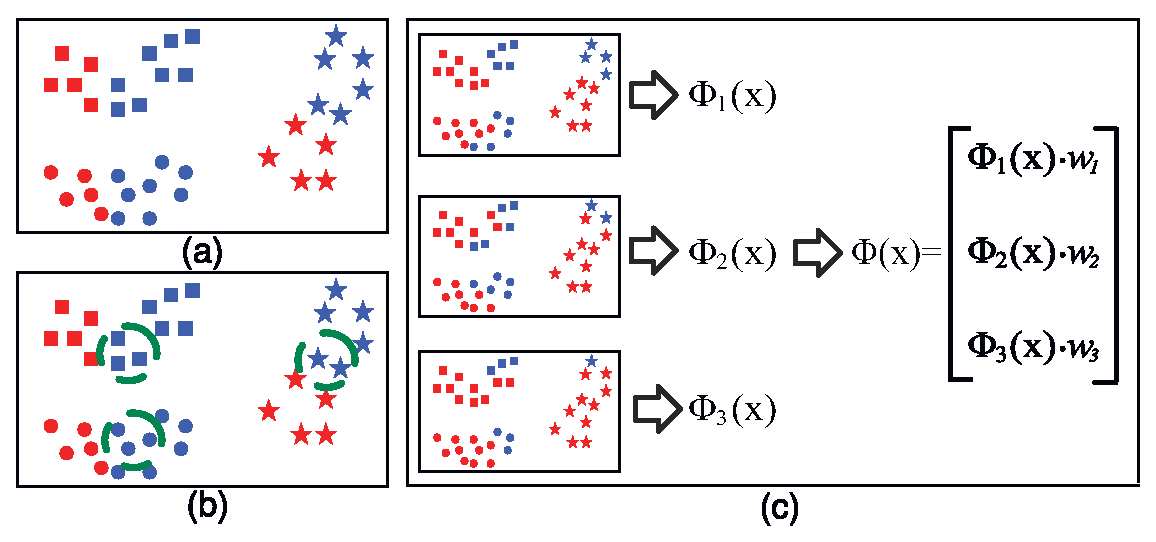
\includegraphics[width=0.8\columnwidth]{fig/fConcept1}
\caption{Main idea of our landmark based approach. (a) The original domain adaptation (DA) problem, where instances in red are from the target and in blue from the source. (b) \textbf{Landmarks}, shown inside the green circles, are data points from the source that can be regarded as samples from the target. (c) Multiple auxiliary tasks are created by augmenting the original target with landmarks, which switch their color (domain association) from blue to red. Each task gives rise to a new feature representation.  These representations are combined discriminatively to form domain-invariant features for the original DA problem. (best viewed in color)}
\label{fConcept}
\end{figure*}


The solutions of the auxiliary tasks give rise to multiple domain-invariant GFKs. We parameterize the invariant features for the original adaptation problem with those resultant kernels.  Intuitively, not all of the kernels are equally useful; to discern which are, we cast the corresponding  learning problem in terms of multiple kernel learning.  We learn the kernel discriminatively to  minimize classification errors on the landmark data instances, which serve as a proxy to discriminative loss on the target domain. Fig.~\ref{fConcept} schematically illustrates the overall approach.

%Despite such progress, existing approaches so far have only been limited to macroscopically examining the distribution similarity by tuning to statistical properties of the samples as a whole --- when comparing distributions, all the samples are used. This notion  is stringent, as it requires all discrepancies to  be accounted for and forces learning inefficiently (or even erroneously) from ``hard'' cases that might be just outliers to the target domains.

%In contrast, we will leverage the key insight that \textbf{\emph{not all instances are created equally in terms of adaptability}}. Thus, we will examine distribution similarity microscopically at the instance level;  In what follows,  we summarize the main idea behind our approach.  After describing it in detail in section~\ref{sApproach}, we contrast it to related work in section~\ref{sRelated}.


%We next describe our three-step landmark based approach. % below: i) identifying and selecting the landmark instances; ii) constructing multiple auxiliary tasks using the landmarks and inferring the corresponding domain-invariant feature spaces, one for each auxiliary task;   iii) discriminatively learning the final domain-invariant feature space that is optimized for the target domain.


\paragraph{\bf Step I: Discovering landmarks} \label{sFindLandmark}

Landmarks are data points from the source domain; however, given how they are distributed, they look like they could be samples from the target domain too (cf. Fig.~\ref{fConcept} for a schematic illustration, and Fig.~\ref{fLandmark} in section~\ref{sExp} for exemplar images identified as landmarks in vision datasets). The intuition behind our approach is to use these landmarks to bridge the source and the target domains.

\emph{How can we identify those landmarks?}  At first glance, it seems that we need to compare all possible subsets of training instances in the source domain to the target. We will show in the following this seemingly intractable problem can be relaxed and solved with tractable convex optimization.

Let $\src=\{(\vct{x}_{m},y_{m})\}_{m=1}^{\cst{M}}$ denote $\cst{M}$ data points and their labels from the source domain. Likewise, we use  $\tgt=\{\vct{x}_{n}\}_{n=1}^{\cst{N}}$ for the target domain.

{\bf Landmark selection.} To identify landmarks, we use  $\cst{M}$ indicator variables $\vct{\alpha}=\{\alpha_m \in \{0,1\}\}$, one for each data point in the source domain. If $\alpha_m = 1$, then $\vct{x}_m$ is regarded as a landmark. Our goal is to choose among all possible configurations of $\vct{\alpha}=\{\alpha_m\}$ such that the distribution of the \textbf{\emph{selected}} data instances is maximally similar to that of the target domain.

To determine whether the two distributions are similar, we use a non-parametric two-sample test called maximum mean discrepancy (MMD)~\cite{gretton2006kernel}. (Other approaches are also possible, including building density estimators when the dimensionality is not high.)  Specifically, we use a nonlinear feature mapping function $\phi(\cdot)$ to map $\vct{x}$ to a Reproducing Kernel Hilbert Space (RKHS) and compare the difference in sample means. {When the mapping function is a unit-ball in a universal RKHS, the difference can be conveniently calculated  in the following\footnote{The unit-ball condition allows the difference to be represented as a metric in the form of eq.~(\ref{eMMD}) and the universality ensures that the means are injective such that the difference in the means is zero if and only if the two distributions are the same. For more analysis, please refer to ~\cite{gretton2006kernel}.},
\begin{equation} \label{eMMD}
\mathsf{MMD}(\vct{\alpha}) = \left\| \frac{1}{\sum_m \alpha_m} \sum_m \alpha_m \phi (\vct{x}_m) - \frac{1}{\cst{N}} \sum_n \phi(\vct{x}_n)\right\|_{\mathcal{H}}^2,
\end{equation}
where $\sum \alpha_m$ is the number of selected landmarks, and the first term  inside the norm is the mean of the selected landmarks under the mapping.  

Our goal is to choose $\vct{\alpha}$ such that the difference is minimized. Furthermore, we impose the constraint that the labels are \emph{balanced} in the selected landmarks. Concretely, we arrive at the following optimization problem,
\begin{align} 
\min_{\vct{\alpha}}  \mathsf{MMD}(\vct{\alpha}) \qquad
\mathsf{s.t.} \quad \frac{1}{\sum_m \alpha_m} \sum_m \alpha_m y_{mc} = \frac{1}{{\cst{M}}}\sum_m y_{mc}, \label{eBalance}
\end{align}
where $y_{mc}$ is an indicator variable for $y_m = c$. The right-hand-side of the constraint is simply the prior probability of the class $c$, estimated from the source.}

We stress that the above criterion is defined on landmarks, which are a \emph{subset} of the source domain, as the sample mean is computed \emph{only} on the selected instances (cf. the denominator $\sum_m \alpha_m$ in eq.~(\ref{eBalance})).  This is very different from other approaches that have used similar non-parametric techniques for comparing distributions~\cite{tca,gretton09kmm}. There they  make stronger assumptions that all data points in the source domain need to be collectively distributed similarly to the target domain.  Furthermore, they do not impose the balance constraint of eq.~(\ref{eBalance}).  Our experimental results  show that these differences are crucial to the success of our approach.

Eq.~(\ref{eBalance}) is intractable due to the binary unknowns $\vct{\alpha}$. We relax and solve it efficiently by introducing new variables $\beta_m$ as $\alpha_m \left(\sum_m \alpha_m\right)^{-1}$.
We relax them to live on the simplex $\Delta=\{\vct{\beta}: \beta_m \ge 0, \sum_m \beta_m=1\}$. Substituting $\{\beta_m\}$ into eq.~(\ref{eBalance}) and its constraints, we arrive at the following {\em quadratic programming problem:}
\begin{equation}
\min_{\vct{\beta} \in \Delta}  \vct{\beta}\T \mat{A}\vct{\beta} - {2}/{\cst{N}}\, \vct{\beta}\T \mat{B} \vct{1} \qquad
\mathrm{ s.t.\ }   \sum_m \beta_m y_{mc} = {1}/{\cst{M}} \sum_m y_{mc},\ \ \ \forall\ c,
\label{eSelected}
\end{equation}
where $\mat{A} \in \R^{\cst{M}\times\cst{M}}$ denotes the positive semidefinite kernel matrix computed over the source domain, and $\mat{B} \in \R^{\cst{M}\times\cst{N}}$ denotes the kernel matrix computed between the source data points and target data points. We recover the binary solution for $\alpha_m$ by  finding the support of $\beta_m$, ie, $\alpha_m = \textsc{threshold}(\beta_m)$. In practice, we often obtain \emph{sparse} solutions, supporting our modeling intuition that only a subset of  instances in the source domain is needed to match the target domain.

{\bf Multiscale analysis.} The selection of landmarks depends on the kernel mapping $\phi(\vct{x})$ and its parameter(s). {To satisfy the requirement of being a unit-ball in a universal RKHS}, we use Gaussian RBF kernels, defined as follows:
\begin{equation} \label{eRBF}
K(\vct{x}_i, \vct{x}_j) = \exp\{  - (\vct{x}_i - \vct{x}_j)\T \mat{M} (\vct{x}_i - \vct{x}_j)/\sigma^2\},
\end{equation}
where the metric $\mat{M}$ is  positive semidefinite and we experiment with several choices.


The bandwidth $\sigma$ is a scaling factor for measuring distances and similarities between data points. Since we regard landmarks as likely samples from the target domain, the bandwidth $\sigma$ determines how much the source and the target are similar to each other at different granularities. A small $\sigma$ will attenuate distances rapidly and regard even close points as being dissimilar. As a result, the algorithm (eq.~(\ref{eBalance})) may select a \emph{large} number of points as landmarks in order to match the target distribution. A large $\sigma$ will have the opposite effect. Fig.~\ref{fLandmark}   illustrates the effect of $\sigma$.

Instead of choosing one scale $\sigma$ in the hope that it fits all, we devise a multiscale approach. We use a set $\{\sigma_q \in [\sigma_{min},\ \sigma_{max}]\}_{q=1}^{\cst{Q}}$. For each $\sigma_q$, we compute the kernel according to eq.~(\ref{eRBF}) and solve eq.~(\ref{eSelected}) to obtain the corresponding landmarks $\mathcal{L}^q = \{ (\vct{x}_m, y_m):  \alpha_m =1\}$.   Using multiple scales  adds the flexibility of modeling data where similarities cannot be measured in one homogeneous scale.  For example, the category of \textsc{grizzly bear} is conceivably much closer to \textsc{grey bear} than to \textsc{polar bear}, so to capture similarities among both the pairs as well as among all three, it is necessary to model them at two scales. Each set of landmarks (one set per scale) gives rise to a different perspective to the adaptation problem by suggesting which instances to explore to connect the source and the target. We achieve this connection by creating auxiliary tasks, as we describe next.

% in the next section, for each cohort of landmarks $\mathcal{L}^q$, we infer a new feature space $\mathcal{Z}^q$ that is domain-invariant if data is examined at the corresponding scale $\sigma^q$. These spaces will be combined nonlinearly and discriminatively to yield a final feature space for domain adaptation (cf. section~\ref{sMKL}).

%We denote all the landmarks collectively  by $\{\landmark\}_{q=1}^\cst{Q}$.  %Intuitively, each $\landmark$ includes the data points from the source which looks like from the target domain, at that scaling.


%In this paper, we focus on using Gaussian RBF style kernels to select landmarks.  Measuring the distance  between $\vct{x}_i$ and $\vct{x}_j$ with respect to a metric $\mat{M}$ as
%\begin{equation}
%d_{\mat{M}}^2 (\vct{x}_i, \vct{x}_j) = (\vct{x}_i - \vct{x}_j)\T \mat{M} (\vct{x}_i - \vct{x}_j),
%\label{eDist}
%\end{equation}
%the corresponding Gaussian kernel uses the bandwidth as a scaling parameter to transferorm distances between data points  into similarity measure

%A large bandwidth $\sigma^2$ will attenuate distances slower and treat distant points being similar. A small bandwidth attenuates distances rapidly and will only treat points in close neighborhood as being similar. In other words, the bandwidth



\paragraph{\bf Step II: Constructing auxiliary tasks} \label{sAuxiliary}
Imagine we create a new source domain $\src^q = \src \setminus \landmark$ and a new target domain $\tgt^q = \tgt\bigcup \landmark$, where the landmarks $\landmark$ are removed from and added to the source and target domains, respectively. The landmarks' labels are not used yet at this stage.

Our auxiliary tasks are defined as $\cst{Q}$  domain adaptation problems, $\src^q \rightarrow \tgt^q$. The auxiliary tasks differ from the original problem $\src \rightarrow \tgt$ in an important aspect:
the new tasks should be ``easier'', as the existence of landmark points ought to aid the adaptation. This is illustrated by the following theorem, stating that the discrepancy between the new domains is smaller than the original.

Let $P_S(X)$ and $P_T(X)$ denote the distributions of the original source and target domains, respectively. Suppose $P_S(X)= \alpha P_N(X) + (1-\alpha)P_L(X)$ with $\alpha \in [0, 1)$ is a mixture model where $P_L(X)$ is the component corresponding to the landmark data points and $P_N(X)$ corresponds to the distribution of the non-landmark instances.  For the auxiliary task, assume the new target distribution is modeled as a mixture distribution $Q_T(X) =  \beta P_T(X) + (1-\beta) P_L(X)$ where $\beta \in [0,\ 1)$. Furthermore, assume the source distribution remains essentially unchanged, which is easily satisfied as long as the number of instances in the source domain is significantly greater than the number of landmark instances and the landmarks are selected \emph{i.i.d.} from $P_L(X)$\footnote{Note that we do not require the landmarks to be \emph{i.i.d} samples from $P_S(X)$ --- they only need to be representative samples of $P_L(X)$.}. In what follows, we omit the arguments $(X)$ to simplify the notation.

\begin{thm}
\label{thAux}
The following inequality holds,
\begin{equation}
 KL( P_S  \|  Q_T ) \le  KL( P_S \|  P_T)  \notag
\end{equation}
where $KL(\cdot\|\cdot)$ stands for the Kullback-Leibler divergence, if %the following condition is satisfied
\begin{align} \label{eAssumption}
\alpha KL(P_N\|P_{T})+(1-\alpha)KL(P_L\|P_{T}) 
    \geq {9}/{8}\max \left\{ KL(P_L\|P_N),\, KL(P_N\|P_L) \right\}.
\end{align}In words, the new target distribution is closer to the source distribution, on the condition that the inter-domain difference (i.e. the left-hand-side) is greater than the intra-domain discrepancy or inhomogeneity (i.e., the right-hand-side).
\end{thm}
The proof is in the Appendix of~\cite{GongIJCV14Learning}. Note that the condition in eq.~(\ref{eAssumption}) is mild:  we expect the source domain is relatively homogeneous and is distinct from the target. With the reduced discrepancy between $P_S(X)$ and $Q_T(X)$, we can apply the analysis in~\cite[Lemma~1]{mansour09multiple} to show that classifiers applied to $Q_T(X)$ attain a smaller generalization error bound than those applied to $P_T(X)$.

These insights motivate our design of auxiliary tasks: they conceivably have low accuracy for binary classification as the landmarks blend the two domains, discouraging the use of domain-specific features.  We describe next how to extract domain-invariant kernels/features using the solutions of those easy problems as a \emph{basis}.

{\bf Learning basis from auxiliary tasks.} {Having shown that the auxiliary tasks represent easier domain adaptation problems, we now use them for adaptation.  Specifically,} for every pair of auxiliary domains, we use the geodesic flow kernel to compute domain-invariant features. The GFK is particularly adept at measuring domain-invariant distances among data points, as exemplified by its superior performance in nearest-neighbor classifiers (cf. section~\ref{sGFKResults}). Thus, it is especially suitable for the final stage of our approach when we compose complex domain-invariant features (cf. section~\ref{sMKL}). The domain-invariant feature space is extracted as the mapping $\Phi_q(\vct{x}) = \mat{L}_q\vct{x}$, where $\mat{G}_q=\mat{L}_q\T\mat{L}_q$ is the GFK for the $q$-th auxiliary task (cf. eq.~(\ref{eGFKInvariant})).  In the following, we describe how to integrate the spaces --- one for each auxiliary task --- \emph{discriminatively} so that the final feature space is optimal for the target.

\paragraph{\bf Step III: Discriminative learning of kernels and classifiers} \label{sMKL}

In this final step, we reveal the second use of landmarks beyond constructing auxiliary tasks. We will use their labels to learn  \emph{discriminative} domain-invariant features for the target domain. Concretely, we compose the features for the original adaptation problem with the auxiliary tasks' features as a basis.

We scale and concatenate those features $\{\sqrt{w_q}\Phi_q(\vct{x})\}_{q=1}^{\cst{Q}}$  into a ``super'' vector $\vct{f}$. Learning $\{w_q\}$ is cast as learning a convex combination of all kernels $\mat{G}_q$ \cite{lanckriet04kernel},
\begin{equation}
\mat{F} = \sum_q w_q \mat{G}_q,\qquad \  \mathrm{s.t.}\ \ \ w_q \ge 0\ \mbox{and}\ \sum_q w_q = 1.
\label{eMKL}
\end{equation}
We use the kernel $\mat{F}$ in training a SVM classifier and the labels of the landmarks $\{\landmark\}$, i.e., $\mkltrain = \sum_q \landmark$ to optimize $\{w_q\}$ discriminatively.  We use $\mkltest = \src \setminus \mkltrain$ as the validation dataset for model selection.  Since $\mkltrain$ consists of landmarks that are distributed similarly to the target, we expect the classification error on $\mkltrain$ to be a good proxy to that of the target.

%Multiple kernel learning formulations such as eq.~(\ref{eMKL}) often yield sparse solutions where some optimal coefficients $w_q$ are zeroes. Thus, the discriminative learning prunes away scales that are not informative. Our experimental results verify that (cf. the Supplementary Material).


\eat{
\subsection{Summary}

To recap our landmark-based approach: i) at each scale $\sigma_q$ and with the aid of GFK, we automatically select \emph{landmark} instances that are distributed similarly to the target; ii) we then construct \emph{auxiliary} tasks and use their solutions as a basis to compose domain-invariant features; iii)  we learn features \emph{discriminatively}, using classification loss on the landmarks as a proxy to the discriminative loss on the target.  %by augmenting the target domain with those landmarks, which aid adaptation. Morever, the solutions to the auxiliary tasks are domain-invariant features that are informative for the original task. iii) those features are discriminatively combined

 in the following: i) for each scale $\sigma_q$,  identify  the set of landmark points $\landmark$ by solving the convex optimization problem eq.~(\ref{eSelected});
ii) for each $\landmark$, construct the corresponding auxiliary task and derive a kernel $\mat{G}_q$ using the method described in section~\ref{sAuxiliary};
iii) formulate the multiple kernel learning problem, and compute the optimal combination coefficients as in eq.~(\ref{eMKL}) to combine the kernels $\mat{G}_q$. The resulting kernel $\mat{F}$ encodes the final domain-invariant feature space.

We emphasize that our approach differs from conventional approaches for learning domain-invariant features \cite{xxx}. In those approaches, invariant features are first learned without using labels and then a classifier is learned with labeled data. One disadvantage of that two-stage paradigm is that the invariant features are \emph{not} optimized to be discriminative. In contrast,
our approach is one-stage:  the combined kernel $\mat{F}$ encodes the invariant features and are trained \emph{discriminatively} with labeled data. Thus, after learning, the domain-invariant features are likely to perform well.
}



%%%%%%%%%%%%%%% OLD TEXT


